\documentclass[../../../../thesis]{subfiles}

\IfEq{\jobname}{\detokenize{thesis}}{}{%
    \setcounterref{chapter}{chap:design}
}


\begin{document}

\section{Module View}\label{sec:module-view}

Phần này tập trung vào các Màn hình, và phân tích chúng theo hướng MVVM.

Trong phần này có dùng nhiều biểu đồ tuần tự (sequence diagram) để minh họa
tương tác của ba thành phần MVVM (cùng với một số thành phần liên quan) trong
các ca sử dụng. Có một số điểm chung về các biểu đồ này:

\begin{itemize}
    \item
        Trừ khi cần thiết, thành phần View sẽ được lược bỏ cho ngắn gọn.
    \item
        Đường thẳng nét đứt thể hiện tính năng data binding (tự động cập nhật
        View), và thường trỏ về ViewModel. Đáng ra, mũi tên này phải trỏ về
        View, nhưng do View bị ẩn đi, nên nó trỏ về ViewModel. Mặc dù không được
        đề cập đến trong phần giới thiệu về MVVM, đây thực ra là một chi tiết
        đúng về mặt kĩ thuật: ViewModel hoàn toàn đọc được luồng dữ liệu gửi đến
        View (hoặc ít nhất là đúng trong cách viết ứng dụng Android thông
        thường).
\end{itemize}

Các biểu đồ trạng thái cũng có một số chi tiết chung:

\begin{itemize}
    \item
        Trừ khi nêu rõ, mọi trạng thái đều có thể là trạng thái bắt đầu (trạng
        thái khi mở ứng dụng) hoặc kết thúc (khi đóng ứng dụng).
    \item
        Mũi tên chuyển trạng thái tương ứng với \emph{tương tác của người dùng},
        do vậy thường được ánh xạ đến một phương thức trong View.
    \item
        Kí hiệu hình tròn đen chỉ dùng để tả trạng thái đầu \emph{khi lần đầu
        dùng} yacv.
\end{itemize}

Biểu đồ lớp thường có một phương thức chung là ``Get InputStream from ID''. Cách
truy cập để lấy \texttt{InputStream} của ảnh từ \texttt{ComicID} có thể tham
khảo từ Màn hình Đọc truyện.


%----------------------------------------------------------------------------------------
%	4.2.1: Nguồn dữ liệu - Repository - DAO - ComicParser
%----------------------------------------------------------------------------------------

\subsection{Nguồn dữ liệu - Repository - DAO - \texttt{ComicParser}}\label{sec:mvvm-design}

Như đã đề cập ở \autoref{chap:fundamental}, yacv sử dụng Kiến trúc Google khuyên
dùng, vốn dựa trên MVVM. Phần này nêu rõ hơn cách triển khai MVVM của yacv trong
phần nguồn dữ liệu (Model/Repository).

Dựa vào \autoref{fig:google-recom-arch}, ta thiết kế được ba nguồn dữ liệu
(model) sau:

\begin{table}[H]
    \centering
    \caption{Ba nguồn dữ liệu tương đương với \autoref{fig:google-recom-arch}}
    \label{tab:3-models}
    \begin{tabular}{l l l}
        \toprule
        Tên                  & Tương đương với    & Mục đích                                              \\
        \midrule
        \texttt{ComicParser} & Remote Data Source & Quét tệp để lấy metadata cập nhật nhất                \\
        DAO                  & Model              & Lấy metadata từ cơ sở dữ liệu, tránh quét đi quét lại \\
        Repository           & Repository         & Tổng hợp hai nguồn trên                               \\
        \bottomrule
    \end{tabular}
\end{table}

Cụ thể hơn, \texttt{ComicParser} là bộ quét metadata tệp truyện (thuộc module
Parser \& Scanner, sẽ được mô tả sau). Lớp này nhận vào URI rồi trả về metadata
của tệp truyện tương ứng dưới dạng đối tượng \texttt{Comic}.

Khi cần đọc dữ liệu metadata từ tệp truyện, ba thành phần này tương tác như sau:

\begin{figure}[H]
    \centering
    \includesvg[scale=0.85,inkscapelatex=false]
        {../images/repo_mvvm_sequence.svg}
    \caption[Tương tác của ba nguồn dữ liệu]{Tương tác của ba nguồn dữ liệu, mũi
        tên gạch đứt thể hiện tính năng data binding}
    \label{fig:3-models}
\end{figure}

Mấu chốt ở đây là \texttt{ComicParser} dù có dữ liệu chính xác (trong trường hợp
một ứng dụng khác sửa metadata tệp truyện) nhưng tốc độ rất chậm, còn cơ sở dữ
liệu không chính xác nhưng rất nhanh, do đó \emph{cơ sở dữ liệu làm bộ đệm cho
    parser}.

Repository làm nhiệm vụ gọi cả hai nguồn dữ liệu trên và cập nhật cơ sở dữ liệu
(nếu cần) thay cho View/ViewModel. Hiện tại, Repository có thể không làm được
nhiều, tuy nhiên nó giúp ích cho \emph{khả năng mở rộng} của ứng dụng. Ví dụ,
trong tương lai yacv có thể liên kết với một bên thứ ba cung cấp metadata cho
truyện, khi đó để tích hợp API thì chỉ cần sửa phần Repository.

Cũng cần chú ý rằng việc đọc metadata từ tệp tin không phải là yêu cầu của mọi
màn hình (cụ thể chỉ Màn hình Metadata cần), do đó trong đa số các ca sử dụng,
\emph{DAO đóng vai trò Model}, thay cho Repository. Tương tác trong
\autoref{fig:3-models} vẫn được duy trì, tuy không có cả Repository lẫn
\texttt{ComicParser}.


%----------------------------------------------------------------------------------------
%	4.2.2: Màn hình Quyền đọc
%----------------------------------------------------------------------------------------

\subsection{Màn hình Quyền đọc}\label{sec:permission-design}

Do sự phức tạp trong việc xin quyền của Android, một màn hình riêng để xin quyền
đọc dữ liệu được tách ra khỏi Màn hình Thư viện, gọi là \emph{Màn hình Quyền
đọc}. Màn hình này sẽ là \emph{màn hình đầu tiên} hiển thị khi dùng ứng dụng.

\begin{itemize}
    \item
        Nếu có quyền đọc: chuyển ngay sang Màn hình Thư viện
    \item
        Nếu không: nêu lí do cần quyền, gợi ý người dùng cấp quyền
\end{itemize}

Hình sau mô tả trạng thái cấp quyền đọc của yacv (cũng như mọi quyền của một ứng
dụng Android cơ bản nói chung).

\begin{figure}[H]
    \centering
    \includegraphics[scale=0.8]{../images/read_permission_state.pdf}
    \caption{Trạng thái cấp quyền của một ứng dụng Android}
    \label{fig:permission-states}
\end{figure}

Dựa theo \autoref{fig:permission-states}, ta có biểu đồ lớp của ViewModel và
View như sau:

\begin{figure}[H]
    \centering
    \includesvg[scale=0.85,inkscapelatex=false]
        {../images/read_permission_mvvm_class.svg}
    \caption{Biểu đồ lớp của Màn hình Quyền đọc}
    \label{fig:read_permission_mvvm_class}
\end{figure}


%----------------------------------------------------------------------------------------
%	4.2.3: Màn hình Thư viện
%----------------------------------------------------------------------------------------

\subsection{Màn hình Thư viện}\label{sec:library-design}

Màn hình Thư viện là một trong hai màn hình của \hyperref[sec:browsing]{ca sử
dụng Duyệt truyện}, bên cạnh Màn hình Thư mục.

Như đã phân tích ở \autoref{sec:scan}, Màn hình Thư viện cần hiển thị cả lỗi và
gợi ý, bên cạnh việc hiển thị danh sách thư mục và chọn thư mục gốc. Do đó, phần
này chia ra làm hai phần con tương ứng.

\subsubsection{Chọn thư mục gốc và hiển thị danh sách thư mục}

Để chọn thư mục gốc, người dùng ấn nút Đổi thư mục gốc để kích hoạt hộp thoại
Chọn thư mục (picker), rồi chọn một thư mục trong đó. Luồng chạy của yacv sẽ
được nêu sau, ở mục riêng về Scanner.

Khi hiển thị danh sách thư mục, cần hiển thị từng phần tử theo tỉ lệ ngang, để
thể hiện tính chất lớn hơn, bao trùm so với tệp truyện trong Màn hình Thư mục.
Do hiển thị theo tỉ lệ ngang mà trang truyện là trang dọc, cần cắt sát phần bên
trên để lấy được phần tên bìa.

% \begin{figure}[H]
%     \centering
%     \includesvg[width=0.8\linewidth,inkscapelatex=false]
%         {../images/scanning_sequence.pdf}
%     \caption{Quét tệp truyện khi thay đổi thư mục gốc và hiển thị}
%     \label{fig:scanning_sequence}
% \end{figure}

\subsubsection{Ngoại lệ trong Màn hình Thư viện}

\begin{wrapfigure}[12]{r}{10cm}
    \centering
    \includegraphics[width=\linewidth]{../images/library_state.pdf}
    \caption{Trạng thái của Màn hình Thư viện}
    \label{fig:library_state}
\end{wrapfigure}

Ngoại lệ ở đây chỉ cả trường hợp không tìm thấy thư mục, lẫn trường hợp không
quét được thư mục vì các lí do đã nêu trong \autoref{sec:scan}. Khi này, ứng
dụng hiển thị một hàng chữ để gợi ý về việc nên làm.

Hình sau là biểu đồ trạng thái, cũng là mô tả về nội dung gợi ý. Riêng trạng
thái ``Có truyện'' là trạng thái hiển thị danh sách thư mục trong luồng cơ bản
đã nêu trên, tức thư mục được hiển thị đầy đủ thay vì chỉ hiện thông báo lỗi.

Tổng hợp lại, ta có biểu đồ lớp của Màn hình Thư viện như sau:

\begin{figure}[H]
    \centering
    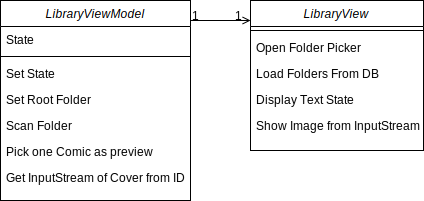
\includegraphics[scale=0.85]{../images/library_mvvm_class.pdf}
    \caption{Biểu đồ lớp của Màn hình Thư viện}
    \label{fig:library_mvvm_class}
\end{figure}

Nhắc lại, cách truy cập để lấy \texttt{InputStream} của ảnh từ \texttt{ComicID}
có thể tham khảo từ Màn hình Đọc truyện.


%----------------------------------------------------------------------------------------
%	4.2.4: Màn hình Thư mục
%----------------------------------------------------------------------------------------

\subsection{Màn hình Thư mục}\label{sec:folder-design}

Màn hình Thư mục là một trong hai màn hình của ca sử dụng Duyệt truyện, bên cạnh
Màn hình Thư viện.

Trong khi phân tích yêu cầu, ta đã phân tích được rằng màn hình hiển thị danh
sách truyện - một phần trong \hyperref[sec:search-comic]{ca sử dụng tìm kiếm} -
phải có giao diện giống Màn hình Thư mục, vì đều hiển thị danh sách truyện. Do
đó, hai màn hình này được gộp lại, gọi chung là \emph{Màn hình Danh sách
truyện}, và sẽ được mô tả sau.


%----------------------------------------------------------------------------------------
%	4.2.5: Màn hình Đọc truyện
%----------------------------------------------------------------------------------------

\subsection{Màn hình Đọc truyện}\label{sec:reader-design}

\begin{wrapfigure}[8]{r}{10cm}
    \centering
    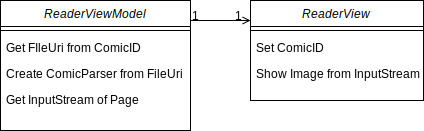
\includegraphics[scale=0.85]{../images/reader_mvvm_class.pdf}
    \caption{Biểu đồ lớp của Màn hình Đọc truyện}
    \label{fig:reader_mvvm_class}
\end{wrapfigure}

Để hiển thị các trang truyện, Màn hình Đọc truyện cần nhận \texttt{ComicID}
(hoặc một đối tượng \texttt{Comic} hoàn chỉnh, tuy nhiên cốt yếu vẫn là thông
tin \texttt{ComicID}) của một tệp truyện, sau đó đưa cho \texttt{ComicParser} để
lấy luồng đọc cho từng trang truyện. \autoref{fig:reader-sequence} là biểu đồ
tuần tự của màn hình này.

Ta cũng có biểu đồ lớp tương ứng trong \autoref{fig:reader_mvvm_class}.

\begin{figure}[H]
    \centering
    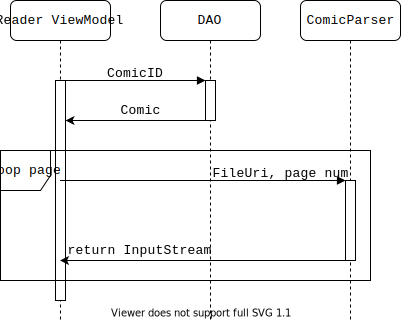
\includegraphics[scale=0.85]{../images/reader_sequence.pdf}
    \caption{Biểu đồ tuần tự của Màn hình Đọc truyện}
    \label{fig:reader-sequence}
\end{figure}


%----------------------------------------------------------------------------------------
%	4.2.6: Màn hình Metadata
%----------------------------------------------------------------------------------------

\subsection{Màn hình Metadata}\label{sec:metadata-design}

Màn hình Metadata tuân theo biểu đồ tuần tự đã nêu ở \autoref{fig:3-models}.
Biểu đồ lớp tương ứng của màn hình này như sau:

\begin{figure}[H]
    \centering
    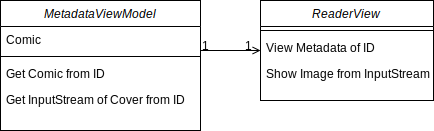
\includegraphics[scale=0.85]{../images/metadata_mvvm_class.pdf}
    \caption{Biểu đồ lớp của Màn hình Metadata}
    \label{fig:metadata_mvvm_class}
\end{figure}


%----------------------------------------------------------------------------------------
%	4.2.7: Màn hình Tìm kiếm
%----------------------------------------------------------------------------------------

\subsection{Màn hình Tìm kiếm}\label{sec:search-design}

Màn hình Tìm kiếm là hai trong ba màn hình của \hyperref[sec:search-comic]{ca sử
dụng tìm kiếm truyện}, bên cạnh Màn hình Danh sách truyện (là tổng quát hóa của
Màn hình Thư mục, đã nhắc ở trên). Màn hình Danh sách truyện sẽ được thiết kế ở
ngay mục sau, còn mục này tập trung vào Màn hình Tìm kiếm.

Không khó để thấy thực ra Màn hình Tìm kiếm Tổng quan và Màn hình Tìm kiếm Chi
tiết thực ra là một màn hình, về mặt thị giác:

\begin{itemize}
    \item
        Điểm giống:

        \begin{itemize}
            \item
                Cả hai cùng hiển thị danh sách.
            \item
                Các phần tử cùng loại trong hai màn hình có cách hiển thị giống
                nhau, chuyển đến các màn hình giống nhau.
        \end{itemize}
    \item
        Điểm khác: Danh sách trong Màn hình Tìm kiếm Tổng quan có \emph{thêm}:

        \begin{itemize}
            \item
                Hiển thị bìa với một số kết quả
            \item
                Có thanh ngăn cách
            \item
                Có nút ``Xem thêm''
        \end{itemize}
\end{itemize}

Do vậy, nếu thiết kế phù hợp, hoàn toàn có thể gộp hai màn hình này. Thiết kế
sau giúp thỏa mãn việc này:

\begin{itemize}
    \item
        Màn hình nhận vào một tham số chứa \emph{câu truy vấn}. Tham số này
        thuộc một trong hai kiểu:

        \begin{itemize}
            \item
                \texttt{QuerySingleType}: chứa câu truy vấn và \emph{một} bảng
                để tìm kiếm
            \item
                \texttt{QueryMultipleTypes}: chứa câu truy vấn và một \emph{danh
                sách} bảng để tìm kiếm
        \end{itemize}

        ``Bảng để tìm kiếm'' thực ra là một số quy định trước, ví dụ nếu là số
        \texttt{0} thì bảng được tìm là \texttt{Comic},\ldots{}
    \item
        ViewModel tìm kiếm dựa vào tham số truy vấn

        \begin{itemize}
            \item
                Nếu tham số là \texttt{QuerySingleType}: truy vấn và hiển thị
                kết quả như thông thường
            \item
                Nếu tham số là \texttt{QueryMultipleTypes}: truy vấn các bảng,
                gộp kết quả lại và thêm kiểu kết quả đặc biệt là
                \emph{Placeholder} và \emph{SeeMore} vào vị trí phù hợp để hiển
                thị lần lượt nhóm kết quả và nút ``Xem thêm''
        \end{itemize}
    \item
        Các kết quả, bao gồm hai dạng kết quả đặc biệt ở trên, cài đặt chung
        giao diện \texttt{Metadata}, để có thể được gộp thành một danh sách
\end{itemize}

Nói ngắn gọn, hai màn hình hiển thị hai danh sách dạng như nhau, nhưng danh sách
cho Màn hình Tổng quan có thêm các phần tử đánh dấu. Ta dùng lại ví dụ về truy
vấn \texttt{Watchmen} ở \autoref{sec:search-comic} để minh họa:

\begin{itemize}
    \item
        Truy vấn \texttt{QueryMultipleTypes} được gửi đến Màn hình Tìm kiếm. Câu
        truy vấn là \texttt{Watchmen}, các bảng cần tìm là mọi bảng.
    \item
        ViewModel tìm \texttt{Watchmen} trong mọi bảng, tìm được:

        \begin{itemize}
            \item
              3 tệp truyện trong bảng \texttt{Comic}
            \item
                2 bộ truyện trong bảng \texttt{Series}
        \end{itemize}
    \item
        Màn hình hiển thị:

        \begin{enumerate}
            \item
                Dòng \texttt{Truyện}, rồi 3 tệp truyện (cùng với ảnh bìa)
            \item
                Dòng \texttt{Bộ\ truyện}, 1 bộ truyện, rồi dòng \texttt{Xem\
                thêm}
        \end{enumerate}
    \item
        Khi ấn vào:

        \begin{itemize}
            \item
                Một trong ba tệp truyện: Sang Màn hình Đọc truyện tương ứng.
            \item
                Một bộ truyện: Sang Màn hình Danh sách truyện, chứa truyện trong
                bộ đó.
            \item
                Nút \texttt{Xem\ thêm}: Sang Màn hình Tìm kiếm, lần này tham số
                là một \texttt{QuerySingleType}, với câu truy vấn là
                \texttt{Watchmen}, còn bảng để tìm là \texttt{Series}. Hai bộ
                truyện kết quả được hiển thị đầy đủ. Chọn một bộ truyện lúc này
                giống với chọn bộ truyện ở trên (sang Màn hình Danh sách
                truyện).
        \end{itemize}
\end{itemize}

Biểu đồ lớp của các đối tượng liên quan như sau:

\begin{figure}[H]
    \centering
    \begin{subfigure}[b]{0.36\textwidth}
        \centering
        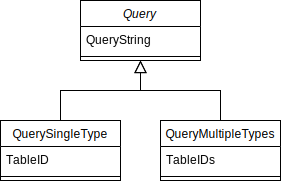
\includegraphics[scale=0.75]{../images/query_class.pdf}
        \caption{Biểu đồ lớp \texttt{Query}}
    \end{subfigure}
    \begin{subfigure}[b]{0.63\textwidth}
        \centering
        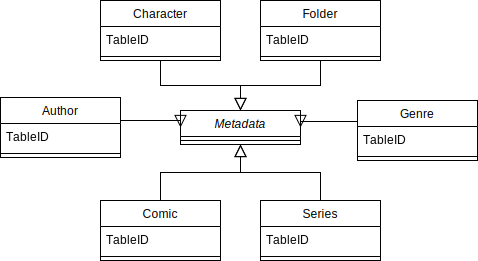
\includegraphics[scale=0.75]{../images/metadata_class.pdf}
        \caption{Biểu đồ lớp \texttt{Metadata}}
    \end{subfigure}
    \caption{Biểu đồ các lớp liên quan đến Màn hình Tìm kiếm}
    \label{fig:graph-related-class}
\end{figure}

Biểu đồ lớp của bản thân Màn hình Tìm kiếm như sau:

\begin{figure}[H]
    \centering
    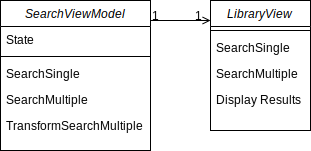
\includegraphics[scale=0.85]{../images/search_mvvm_class.pdf}
    \caption{Biểu đồ lớp của Màn hình Tìm kiếm}
    \label{fig:search_mvvm_class}
\end{figure}

Do mỗi DAO trả kết quả của bảng tương ứng về ở dạng danh sách, nên khi dùng
\texttt{QueryMultipleTypes}, các danh sách kết quả lẻ này tổng hợp, và thêm hai
kiểu kết quả đặc biệt. Hàm \texttt{TransformSearchMultiple()} là để ``làm
phẳng'' mảng kết quả hai chiều như trên.


%----------------------------------------------------------------------------------------
%	4.2.7: Màn hình Danh sách truyện
%----------------------------------------------------------------------------------------

\subsection{Màn hình Danh sách truyện}\label{sec:list-comic-design}

Màn hình này là màn hình thứ ba trong chuỗi các màn hình liên quan đến ca sử
dụng tìm kiếm, đồng thời đóng vai trò của Màn hình Thư mục (do là phiên bản tổng
quát hơn của nó).

Màn hình này nhận vào một tham số kiểu \texttt{Metadata} thay vì một
\texttt{Query}, và trả về danh sách các \emph{tệp truyện} - \texttt{Comic} - có
liên kết với tham số đầu vào.

Khi hiển thị danh sách tệp truyện, cần hiển thị từng phần tử theo tỉ lệ dọc,
khác với tỉ lệ ngang của phần tử thư mục trong \hyperref[sec:library-design]{Màn
hình Thư viện}. Do hiển thị theo chiều dọc, mà trang truyện cũng dọc, cần thu
nhỏ kích cỡ phần tử bằng cách một dòng cho hiển thị 2-3 phần tử.

Biểu đồ lớp của Màn hình Danh sách truyện như sau:

\begin{figure}[H]
    \centering
    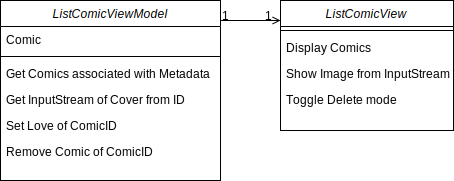
\includegraphics[scale=0.85]{../images/list_comics_mvvm_class.pdf}
    \caption{Biểu đồ lớp của Màn hình Danh sách truyện}
    \label{fig:list_comics_mvvm_class}
\end{figure}

\end{document}
